\section{VedAnvaya as a Research Interface}
\label{sec:interface}

The graph is exposed through a read-only \mbox{API} and a web interface called
VedAnvaya. We treat it here as evidence for one narrow claim --- that the evidence
typing survives into use --- rather than as a contribution in its own right.

The design constraint that matters is that typing is rendered \emph{at the point of
reading}, not collected on a methods page. \Cref{fig:product} shows the effect on a
single S\=amavedic verse. Four distinct epistemic situations are visible
simultaneously, each labelled in place: the svara marks are shown with the note that
they are reproduced exactly as the source edition prints them, are a record of that
edition's notation rather than a reconstructed melody, and that nothing derives a
sung realisation from them; the English is labelled a rendering \emph{via} the
verified \d{R}gvedic parallel, with a scope note stating that it is not an
independent translation of this corpus and is excluded from its translated count;
the deity named inside the verse is marked \code{PROBABLE} rather than asserted; and
the traditional ascription is marked ``not yet modelled'' rather than omitted.

\begin{figure}[tbp]
\centering
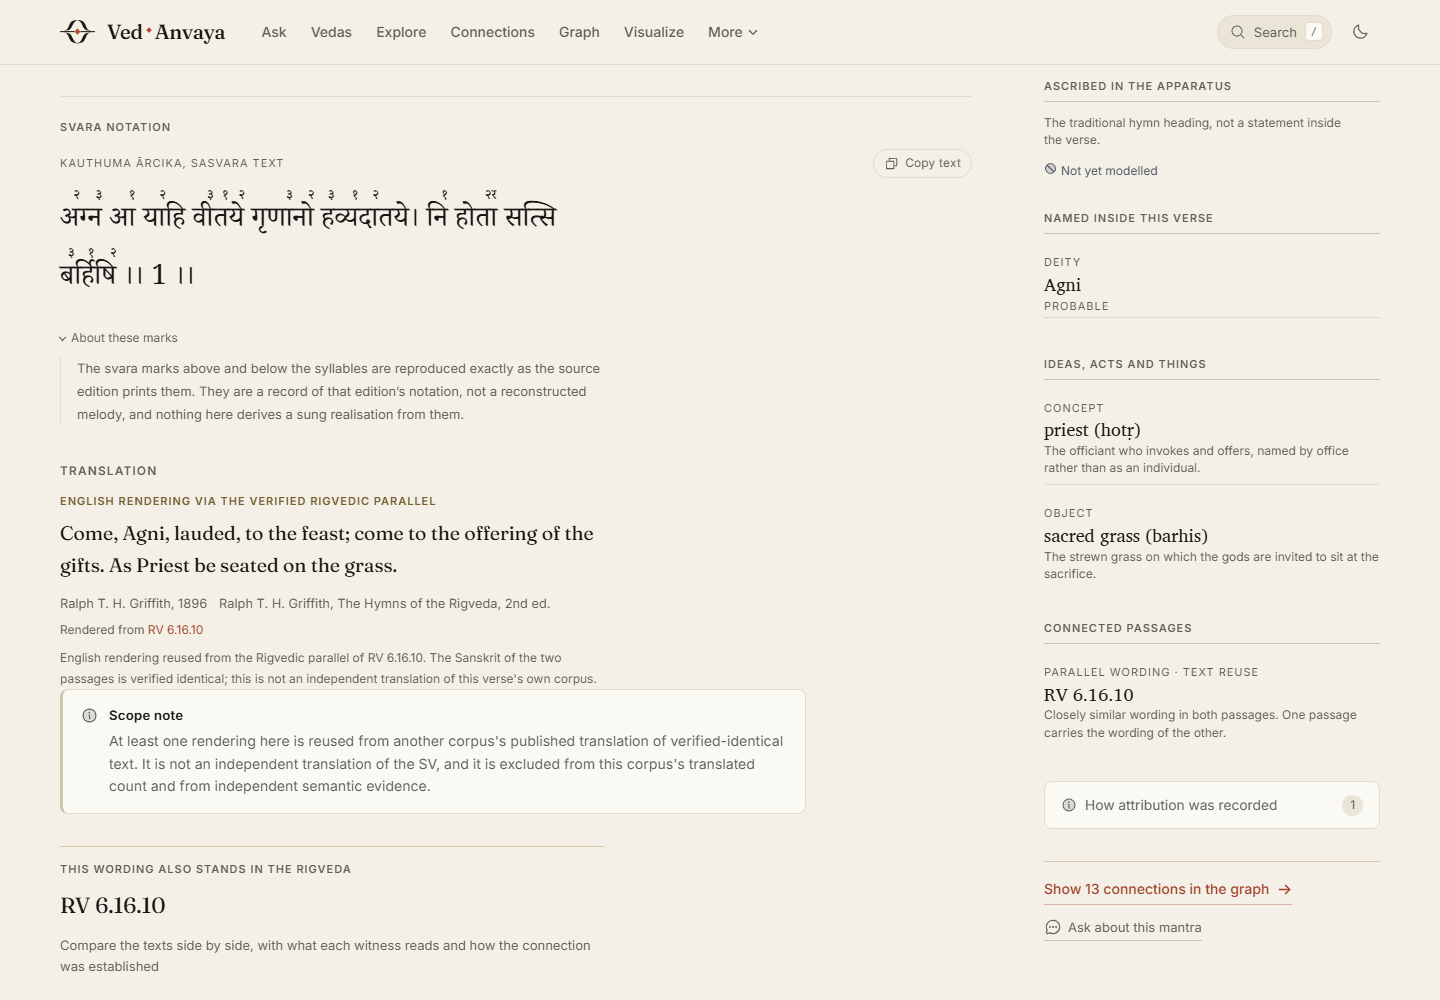
\includegraphics[width=0.96\linewidth]{figures/product/reader-samaveda-notation.png}

\vspace{6pt}
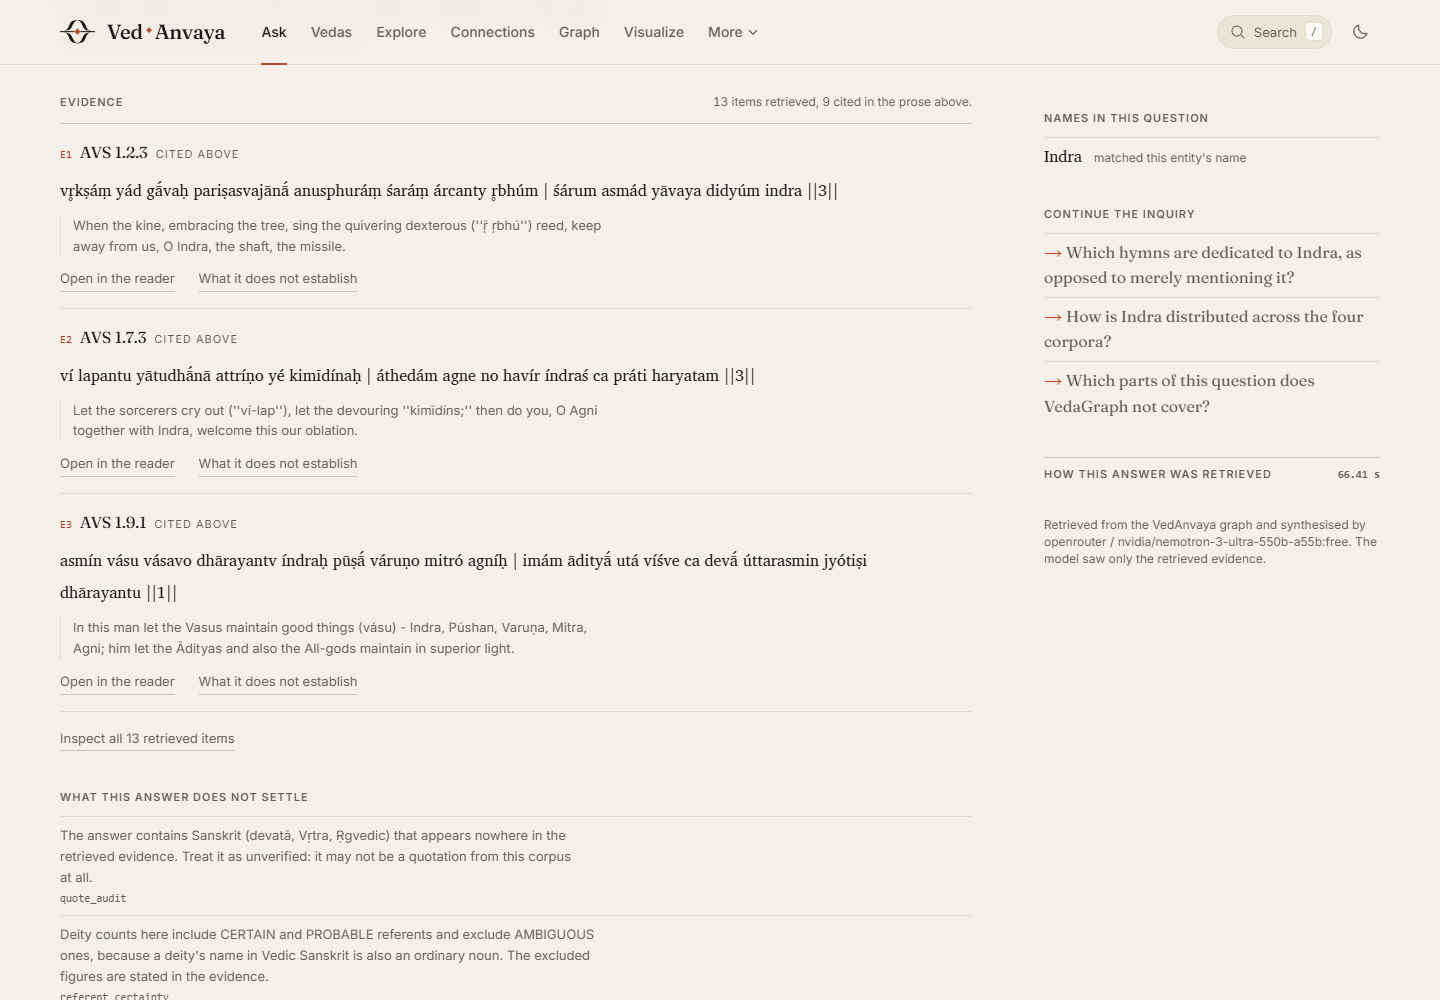
\includegraphics[width=0.96\linewidth]{figures/product/ask-evidence.png}
\caption{Evidence typing rendered where the reader is. \textbf{Top:} one
S\=amavedic verse showing four epistemic situations at once --- source-explicit
svara marks with the note that they are a record of the edition's notation and not a
reconstructed melody; an English rendering labelled as reused via a verified
\d{R}gvedic parallel and excluded from this corpus's translated count; a deity named
inside the verse marked \code{PROBABLE}; and a traditional ascription marked ``not
yet modelled'' rather than omitted. \textbf{Bottom:} the retrieved evidence beside a
synthesised answer, with a per-item ``what it does not establish'' affordance and a
closing section populated by the mechanical auditors rather than by the model.
Captured from the running product against the graph census this paper reports.}
\label{fig:product}
\end{figure}

The same discipline governs synthesis. The question-answering surface displays the
retrieved evidence beside the prose, gives each cited item an
``\emph{what it does not establish}'' affordance, and closes with a section headed
``what this answer does not settle'' that is populated by the mechanical auditors
rather than by the model --- in the case shown, a warning that the answer contains
Sanskrit appearing nowhere in the retrieved evidence, and a note that the deity
counts quoted include certain and probable referents and exclude ambiguous ones
because a deity's name in Vedic Sanskrit is also an ordinary noun.

Two behaviours are worth recording because they are unusual for an interface of this
kind and both follow from the graph rather than from interface design. The
question-answering layer declines 17 of 60 benchmark questions as insufficiently
evidenced (\cref{sec:eval-ask}). And a corpus page reports coverage as four
populations rather than one percentage, so that the S\=amaveda's zero independent
English translations is legible next to its 173 reused renderings instead of being
averaged into a single figure that would be true of neither.

We also report the interface's most instructive failure, because it is a
graph-level lesson. Restoring 30{,}266 semantic-assertion nodes --- a correct
restoration of real data --- pushed the share of the exported public graph that is
apparatus rather than entity to roughly 81\,\%, so that a visualisation of Indra's
neighbourhood at a fixed budget spent 21 of 40 slots on passages and evidence
records and 6 on other deities. Nothing had become false; the graph had simply
stopped being legible at that budget. The repair was per-class display ceilings, not
a change to the data. Completeness and legibility are different objectives, and an
interface over an evidence-typed graph has to be designed for both
(\cref{sec:failure}, F6).
